\documentclass[twoside, final]{hcmut_report}
% \usepackage{codespace}
% Configuration
\upperuniname{ĐẠI HỌC QUỐC GIA THÀNH PHỐ HỒ CHÍ MINH}
\uniname{TRƯỜNG ĐẠI HỌC BÁCH KHOA}
\deptname{KHOA KHOA HỌC VÀ KỸ THUẬT MÁY TÍNH}

\coursename{XÁC SUẤT VÀ THỐNG KÊ}
\reporttype{BÁO CÁO BÀI TẬP LỚN}
\title{PHÂN TÍCH BỘ DỮ LIỆU VỀ SẢN PHẨM CỦA CỬA HÀNG ĐIỆN TỬ TRỰC TUYẾN}
\advisor{
    TS. Phan Thị Hường
}
\student{
    Trần Điền Minh          ,   2312116
    Phan Thanh Sơn          ,   2312975
    Nguyễn Hoàng Anh Thắng  ,   2313185
    Huỳnh Văn Lợi           ,   2311974
    Cao Chí Nguyên          ,   2312331
    Nguyễn Hữu Thịnh        ,   2313292
}

\begin{document}
\begin{titlepage}
    \coverpage
    \newpage
    \begin{center}
        \small \bfseries 
        BÁO CÁO PHÂN CÔNG NHIỆM VỤ VÀ KẾT QUẢ THỰC HIỆN ĐỀ TÀI         
        
        NHÓM: 10 -- LỚP: TN01 -- HỌC KỲ: 241 -- MÔN: XÁC SUẤT VÀ THỐNG KÊ   
    \renewcommand{\arraystretch}{1.2}
    \begin{table}[h!]
        \centering
        \resizebox{\textwidth}{!}{%
        \begin{tabular}{|c|l|c|l|c|c|}
            \hline
            \textbf{STT} & \textbf{Họ và tên}         & \textbf{MSSV}   & \textbf{Nhiệm vụ}                             & \textbf{Đóng góp} & \textbf{Điểm chia $\pm 2$} \\ \hline
            1            & Trần Điền Minh            & 2312116         & Hồi quy đa bội                                 & 100 \% & 0 \\ \hline
            2            & Phan Thanh Sơn            & 2312975         & \makecell[l]{Kiểm định hai mẫu \\ \& một mẫu}  & 100 \% & 0 \\ \hline
            3            & Nguyễn Hoàng Anh Thắng    & 2313185         & Anova hai nhân tố                              & 100 \% & 0 \\ \hline
            4            & Huỳnh Văn Lợi             & 2311974         & Anova một nhân tố                              & 100 \% & 0 \\ \hline
            5            & Cao Chí Nguyên            & 2312331         & Thực hiện thống kê mô tả                       & 100 \% & 0 \\ \hline
            6            & Nguyễn Hữu Thịnh          & 2313292         & Thực hiện tiền xử lí số liệu                   & 100 \% & 0 \\ \hline
        \end{tabular}
        }        
    \end{table}
\end{center}
    \newpage
    \tableofcontents
    \newpage
\end{titlepage}

\setcounter{page}{1}
\pagestyle{empty}

\pagestyle{fancy}
\pagebreak
\section{Tổng quan dữ liệu}
\subsection{Mô tả dữ liệu}
Tập dữ liệu được cung cấp trong BTL chứa thông tin về một cửa hàng điện tử trực tuyến. Cửa hàng có ba kho hàng hóa để giao hàng cho khách hàng. Dựa vào dữ liệu đã cho để tìm mối quan hệ giữa các biến, từ đó xây dựng mô hình giúp hiểu rõ những yếu tố ảnh hưởng đến giá trị của tổng đơn hàng.

\begin{itemize}
    \item Tiêu đề: Transactional Retail Dataset of Electronics Store
    \item Thông tin nguồn:
        \begin{itemize}
            \item Tác giả: SHAHRAYAR
            \item Thời điểm công bố dữ liệu: 3 năm trước
        \end{itemize}
    \item Giá trị quan trắc: 500
    \item Số lượng biến: 16
\end{itemize}
Trong bài tập lớn này, nhóm đã quyết định sử dụng file \textbf{dirty\_data.csv} để làm dữ liệu cho việc xây dựng các mô hình thống kê.
\subsection{Mô tả biến}
Dữ liệu dưới đây được thu thập và tổ chức nhằm mục đích hỗ trợ quá trình phân tích và quản lý đơn hàng trong hệ thống thương mại điện tử. Đây là tập hợp các thông tin chi tiết liên quan đến đơn đặt hàng, khách hàng, sản phẩm, và các yếu tố khác có liên quan.

Các biến được chia thành hai dạng tương ứng:
\begin{itemize}
    \item \textbf{7 biến phân loại:} order\_id, customer\_id, nearest\_warehouse, season, is\_expedited\_delivery, latest\_customer\_review, is\_happy\_customer.
    \item \textbf{6 biến liên tục:} order\_price, delivery\_charges, customer\_lat, customer\_long, coupon\_discount, order\_total, distance\_to\_nearest\_warehouse. 
\end{itemize}

Mỗi biến trong bảng dữ liệu đều được mô tả một cách cụ thể, bao gồm: Tên biến, loại dữ liệu, đơn vị đo lường (nếu có), và ý nghĩa của biến.
Các thông tin này giúp làm rõ bản chất và vai trò của từng trường dữ liệu trong hệ thống. Dữ liệu này không chỉ hỗ trợ phân tích các xu hướng mua hàng mà còn cung cấp các thông tin quan trọng để dự đoán nhu cầu, tối ưu hóa chi phí vận hành và cải thiện trải nghiệm khách hàng. Bảng dưới đây trình bày chi tiết từng biến, được tổ chức theo từng nhóm thông tin cụ thể, giúp người đọc dễ dàng tiếp cận và hiểu rõ hơn về dữ liệu được sử dụng.

\vspace{0.5cm}

% Row 1
\noindent
\begin{minipage}[t]{0.48\textwidth}
\begin{mainbox}{Biến 1: order\_id}{1}
    \textbf{Loại dữ liệu:} Chuỗi kí tự \\
    \textbf{Đơn vị:} (Trống) \\
    \textbf{Mô tả:} Một ID duy nhất cho mỗi đơn hàng.
\end{mainbox}
\end{minipage}
\hfill
\begin{minipage}[t]{0.48\textwidth}
\begin{mainbox}{Biến 2: customer\_id}{1}
    \textbf{Loại dữ liệu:} Chuỗi kí tự \\
    \textbf{Đơn vị:} (Trống) \\
    \textbf{Mô tả:} Một ID duy nhất cho mỗi khách hàng.
\end{mainbox}
\end{minipage}

\vspace{0.5cm}

% Row 2
\noindent
\begin{minipage}[t]{0.48\textwidth}
\begin{mainbox}{Biến 3: date}{2}
    \textbf{Loại dữ liệu:} Chuỗi kí tự \\
    \textbf{Đơn vị:} (Trống) \\
    \textbf{Mô tả:} Ngày đặt hàng, được đưa ra ở định dạng YYYY-MM-DD.
\end{mainbox}
\end{minipage}
\hfill
\begin{minipage}[t]{0.48\textwidth}
\begin{mainbox}{Biến 4: nearest\_warehouse}{2}
    \textbf{Loại dữ liệu:} Chuỗi kí tự \\
    \textbf{Đơn vị:} (Trống) \\
    \textbf{Mô tả:} Một chuỗi biểu thị tên của kho hàng gần nhất với khách hàng.
\end{mainbox}
\end{minipage}

\vspace{0.5cm}

% Row 3
\noindent
\begin{minipage}[t]{0.48\textwidth}
\begin{mainbox}{Biến 5: shopping\_cart}{3}
    \textbf{Loại dữ liệu:} Chuỗi kí tự \\
    \textbf{Đơn vị:} (Trống) \\
    \textbf{Mô tả:} Một danh sách các bộ đại diện cho các hạng mục trong đơn hàng: phần tử đầu tiên của bộ dữ liệu là mục được sắp xếp và phần tử thứ hai là số lượng đặt hàng cho mặt hàng đó.
\end{mainbox}
\end{minipage}
\hfill
\begin{minipage}[t]{0.48\textwidth}
\begin{mainbox}{Biến 6: order\_price}{3}
    \textbf{Loại dữ liệu:} \(x \in (0; +\infty)\) \\
    \textbf{Đơn vị:} USD \\
    \textbf{Mô tả:} Một số biểu thị giá đặt hàng bằng USD. Giá đặt hàng là giá của các mặt hàng trước khi có bất kỳ khoản giảm giá và/hoặc phí giao hàng nào được áp dụng.
\end{mainbox}
\end{minipage}

\vspace{0.5cm}

% Row 4
\noindent
\begin{minipage}[t]{0.48\textwidth}
\begin{mainbox}{Biến 7: delivery\_charges}{4}
    \textbf{Loại dữ liệu:} \(y \in (0; +\infty)\) \\
    \textbf{Đơn vị:} USD \\
    \textbf{Mô tả:} Một số thể hiện phí giao hàng của đơn hàng.
\end{mainbox}
\end{minipage}
\hfill
\begin{minipage}[t]{0.48\textwidth}
\begin{mainbox}{Biến 8: customer\_lat}{4}
    \textbf{Loại dữ liệu:} \(z \in (-90; 90)\) \\
    \textbf{Đơn vị:} Độ \\
    \textbf{Mô tả:} Vĩ độ vị trí của khách hàng.
\end{mainbox}
\end{minipage}

\vspace{0.5cm}

% Row 5
\noindent
\begin{minipage}[t]{0.48\textwidth}
\begin{mainbox}{Biến 9: customer\_long}{5}
    \textbf{Loại dữ liệu:} \(t \in (-180; 180)\) \\
    \textbf{Đơn vị:} Độ \\
    \textbf{Mô tả:} Kinh độ vị trí của khách hàng.
\end{mainbox}
\end{minipage}
\hfill
\begin{minipage}[t]{0.48\textwidth}
\begin{mainbox}{Biến 10: coupon\_discount}{5}
    \textbf{Loại dữ liệu:} \(m \in \mathbb{N}, 0 \leq m \leq 100\) \\
    \textbf{Đơn vị:} \% \\
    \textbf{Mô tả:} Một số nguyên biểu thị phần trăm giảm giá được áp dụng cho đơn giá.
\end{mainbox}
\end{minipage}

\vspace{0.5cm}

% Row 6
\noindent
\begin{minipage}[t]{0.48\textwidth}
\begin{mainbox}{Biến 11: order\_total}{6}
    \textbf{Loại dữ liệu:} \(n \in (0; +\infty), n \leq x\) \\
    \textbf{Đơn vị:} USD \\
    \textbf{Mô tả:} Một số biểu thị tổng giá tiền đơn đặt hàng bằng USD, giảm giá và/hoặc phí giao hàng đã được áp dụng.
\end{mainbox}
\end{minipage}
\hfill
\begin{minipage}[t]{0.48\textwidth}
\begin{mainbox}{Biến 12: season}{6}
    \textbf{Loại dữ liệu:} Chuỗi kí tự \\
    \textbf{Đơn vị:} (Trống) \\
    \textbf{Mô tả:} Một chuỗi biểu thị mùa mà đơn hàng được đặt.
\end{mainbox}
\end{minipage}

\vspace{0.5cm}

% Row 7
\noindent
\begin{minipage}[t]{0.48\textwidth}
\begin{mainbox}{Biến 13: is\_expedited\_delivery}{7}
    \textbf{Loại dữ liệu:} \(t = \text{TRUE}\) (có), \(t = \text{FALSE}\) (không) \\
    \textbf{Đơn vị:} (Trống) \\
    \textbf{Mô tả:} Một hàm nhị phân biểu thị liệu khách hàng có yêu cầu giao hàng nhanh hay không.
\end{mainbox}
\end{minipage}
\hfill
\begin{minipage}[t]{0.48\textwidth}
\begin{mainbox}{Biến 14: distance\_to\_nearest\_warehouse}{7}
    \textbf{Loại dữ liệu:} \(r \in (0; +\infty)\) \\
    \textbf{Đơn vị:} km \\
    \textbf{Mô tả:} Một số biểu thị khoảng cách vòng cung, tính bằng km, giữa khách hàng và kho hàng gần nhất với họ.
\end{mainbox}
\end{minipage}

\vspace{0.5cm}

% Row 8
\noindent
\begin{minipage}[t]{0.48\textwidth}
\begin{mainbox}{Biến 15: latest\_customer\_review}{8}
    \textbf{Loại dữ liệu:} Chuỗi kí tự \\
    \textbf{Đơn vị:} (Trống) \\
    \textbf{Mô tả:} Một chuỗi đại diện cho đánh giá mới nhất của khách hàng về đơn hàng gần đây nhất của họ.
\end{mainbox}
\end{minipage}
\hfill
\begin{minipage}[t]{0.48\textwidth}
\begin{mainbox}{Biến 16: is\_happy\_customer}{8}
    \textbf{Loại dữ liệu:} \(q = \text{TRUE}\) (có), \(q = \text{FALSE}\) (không) \\
    \textbf{Đơn vị:} (Trống) \\
    \textbf{Mô tả:} Một hàm nhị phân biểu thị liệu khách hàng có hài lòng hay không? Hoặc gặp vấn đề với đơn hàng gần đây nhất của họ.
\end{mainbox}
\end{minipage}
\section{Kiến thức nền}\label{Kien thuc nen}
\subsection{Thống kê mô tả}
Phương pháp thống kê mô tả (descriptive statistics) là một phương pháp trong khoa học thống kê được sử dụng để mô tả và tóm tắt các dữ liệu một cách đơn giản và dễ hiểu. Phương pháp này giúp chúng ta hiểu thông tin cơ bản về các biến trong dữ liệu mà không cần đưa ra các phán đoán hay suy luận về mối quan hệ giữa các biến. Các phương pháp thống kê mô tả thường bao gồm các đại lượng thống kê như \textbf{giá trị trung bình, phương sai, độ lệch chuẩn, phân vị, tỉ lệ phần trăm, đồ thị và biểu đồ}. Các đại lượng này giúp chúng ta hiểu về trung tâm, phân tán và hình dạng của dữ liệu.
\subsection{Thống kê suy diễn}
Trong bài tập lớn này, nhóm có vận dụng những kiến thức được học trên lớp như xây dựng khoảng tin cậy, kiểm định giả thuyết, định lý giới hạn trung tâm, v.v... Tuy nhiên, 
\subsubsection{Phân tích phương sai 2 nhân tố}
Phân tích phương sai 2 nhân tố (Two-Way ANOVA) là một phương pháp thống kê được sử dụng để kiểm tra sự ảnh hưởng của hai yếu tố (hay còn gọi là biến độc lập) đến một biến phụ thuộc (biến kết quả), cũng như mối quan hệ tương tác giữa chúng.

Giả sử có hai yếu tố \textit{A} và \textit{B}, với các mức độ tương ứng là a và b. Mô hình phân tích phương sai 2 nhân tố được xây dựng như sau:
\[
Y_{ijk} = \mu + \alpha_i + \beta_j + (\alpha \beta)_{ij} + \epsilon_{ijk}
\]
Trong đó:
\begin{itemize}
  \item \( Y_{ijk} \): giá trị quan sát thứ \( k \) của tổ hợp mức độ \( i \) của yếu tố \( A \) và mức độ \( j \) của yếu tố \( B \).
  \item \( \mu \): giá trị trung bình tổng thể.
  \item \( \alpha_i \): hiệu ứng của mức độ \( i \) của yếu tố \( A \).
  \item \( \beta_j \): hiệu ứng của mức độ \( j \) của yếu tố \( B \).
  \item \( (\alpha\beta)_{ij} \): hiệu ứng tương tác giữa yếu tố \( A \) và \( B \).
  \item \( \epsilon_{ijk} \): sai số ngẫu nhiên (residual).
\end{itemize}
\subsection{Hồi quy tuyến tính đa bội}
Hồi quy tuyến tính đa biến là một phương pháp thống kê được sử dụng để mô hình hóa mối quan hệ giữa một biến phụ thuộc (hay còn gọi là biến mục tiêu) và một hoặc nhiều biến độc lập (biến giải thích). Mục tiêu của hồi quy tuyến tính đa biến là dự đoán giá trị của biến phụ thuộc dựa trên các giá trị của các biến độc lập.

Mô hình hồi quy tuyến tính đa biến có dạng:

\[
Y = \beta_0 + \beta_1 X_1 + \beta_2 X_2 + \dots + \beta_p X_p + \epsilon
\]

Trong đó:
\begin{itemize}
  \item \(Y\) là biến phụ thuộc (biến mục tiêu).
  \item \(X_1, X_2, \dots, X_p\) là các biến độc lập (biến giải thích).
  \item \(\beta_0\) là hệ số chặn (intercept), đại diện cho giá trị của \(Y\) khi tất cả các biến độc lập đều bằng 0.
  \item \(\beta_1, \beta_2, \dots, \beta_p\) là các hệ số hồi quy (coefficient) đại diện cho mức độ tác động của mỗi biến độc lập đến biến phụ thuộc.
  \item \(\epsilon\) là sai số ngẫu nhiên (error term), thể hiện phần sai khác giữa giá trị thực tế của \(Y\) và giá trị dự đoán.
\end{itemize}

\textbf{Phương pháp bình phương tối thiểu (Ordinary Least Squares - OLS)}: Là phương pháp phổ biến nhất để ước lượng các hệ số \(\beta\) trong hồi quy tuyến tính. Mục tiêu là tìm giá trị của \(\beta\) sao cho tổng bình phương sai số (\(\epsilon\)) là nhỏ nhất.
  
\[
\text{Minimize } \sum_{i=1}^{n} (Y_i - (\beta_0 + \beta_1 X_{i1} + \dots + \beta_p X_{ip}))^2
\]

Sau khi ước lượng các hệ số \(\beta\), chúng ta cần kiểm tra chất lượng mô hình bằng các chỉ số và kiểm định thống kê:

\textbf{R-squared (R²)}: Là một chỉ số đo lường mức độ phù hợp của mô hình với dữ liệu. R² có giá trị từ 0 đến 1, với 1 nghĩa là mô hình giải thích hoàn toàn biến thiên của dữ liệu.
  
  \[
  R^2 = 1 - \frac{\sum (Y_i - \hat{Y}_i)^2}{\sum (Y_i - \bar{Y})^2}
  \]
  
  Trong đó:
  \begin{itemize}
    \item \(\hat{Y}_i\) là giá trị dự đoán từ mô hình.
    \item \(\bar{Y}\) là giá trị trung bình của \(Y\).
  \end{itemize}

\textbf{Kiểm định F}: Kiểm tra xem mô hình hồi quy có giải thích đáng kể biến thiên của dữ liệu hay không.

\textbf{Kiểm định t}: Kiểm tra sự có mặt của mỗi hệ số hồi quy \(\beta_i\), tức là xem mỗi biến độc lập có ảnh hưởng đáng kể đến biến phụ thuộc hay không.

\section{Tiền xử lý số liệu}
\subsection{Đọc dữ liệu}
Để đọc dữ liệu từ tệp tin dirty\_data.csv, ta sử dụng lệnh \textbf{read.csv()} với input là đường dẫn đến tệp tin chứa dữ liệu cần phân tích. Sau đó, ta sử dụng lệnh \textbf{dim()} để hiển thị số hàng \& số cột cùng với lệnh \textbf{names()} để liệt kê các tên biến có trong dữ liệu. Kết quả có được như trong 


\section{Thống kê mô tả}
\subsection{Phân tích và phân chia số liệu}
Sau khi thực hiện bước tiền xử lí số liệu, ta đã làm sạch và điền khuyết dữ liệu, ta thực hiện thống kê mô tả bằng lệnh \texttt{summary()} ta sẽ có cái nhìn tổng quát hơn về bảng dữ liệu. Lệnh \texttt{summary()} sẽ xuất ra màn hình những giá trị như \textit{min} (giá trị nhỏ nhất), \textit{mean} (trung bình), \textit{median} (trung vị), \textit{Q1} (khoảng tứ phân vị thứ 1), \textit{Q3} (khoảng tứ phân vị thứ 3), \textit{max} (giá trị lớn nhất).
\begin{figure}[H]
    \centering
    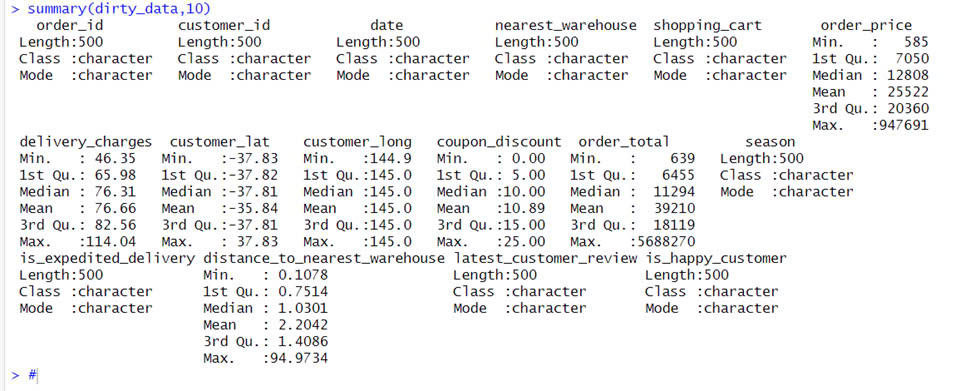
\includegraphics[width=0.9\linewidth]{graphics/bang1.jpg}
    \caption{Số liệu tổng quát}
    
\end{figure}
Sau đó ta chọn lọc những biến có thể phân tích như nearest\_warehouse, order\_price, delivery\_charges, customer\_lat, customer\_long, coupon\_discount, order\_total, season, is\_expedited\_delivery, distance\_to-\\\_nearest\_warehouse, is\_happy\_customer. Và ta có bảng dữ liệu từ lệnh \texttt{head()}.
\begin{figure}[H]
    \centering
    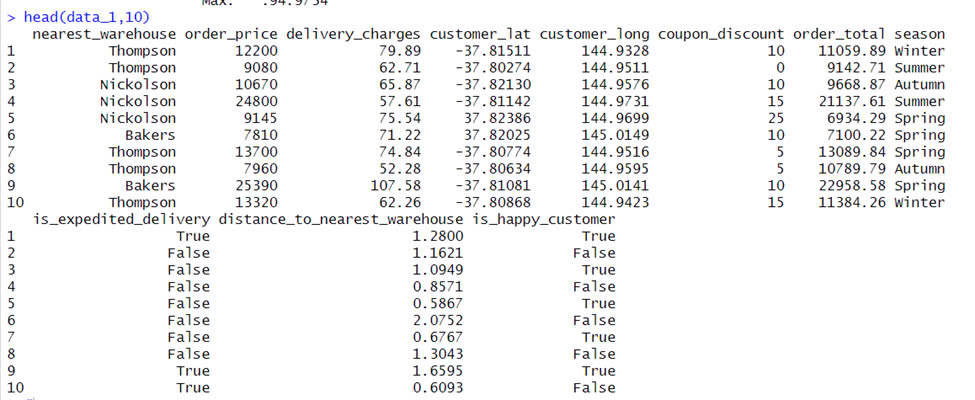
\includegraphics[width=0.9\linewidth]{graphics/bang2.jpg}
    \caption{Số liệu chọn lọc}
   
\end{figure}
            
Từ nội dung của bảng dữ liệu trên, ta tách ra thành:\\
•  Biến liên tục gồm: order\_price, delivery\_charges, customer\_lat, customer\_long, coupon\_discount, order\_total, distance\_to\_nearest\_warehouse.
 \begin{figure}[H]
    \centering
    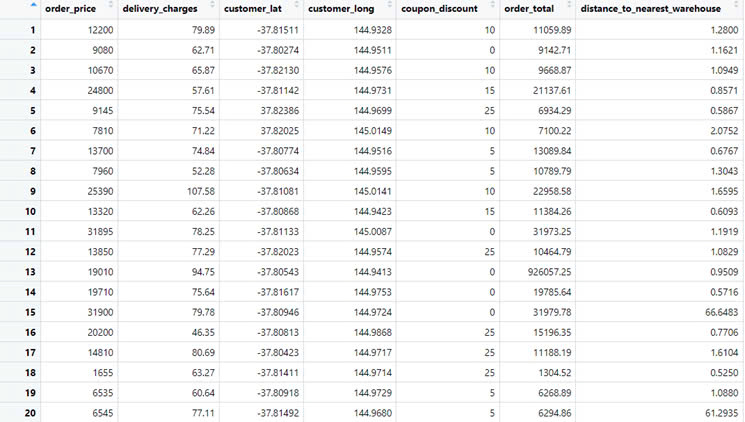
\includegraphics[width=0.9\linewidth]{graphics/bang3.jpg}
    \caption{Các biến liên tục}
   
\end{figure}
•  Biến định lượng gồm: nearest\_warehouse, season, is\_expedited\_delivery, is\_happy\_customer. Và biến định lượng được biểu diễn dưới dạng factor như sau.
\begin{figure}[H]
    \centering
    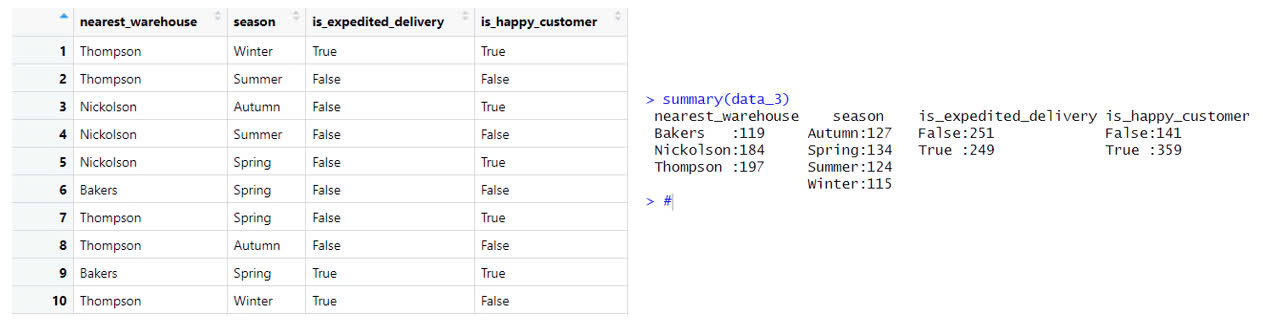
\includegraphics[width=0.9\linewidth]{graphics/bang6.jpg}
    \caption{Các biến định lượng và giá trị được biểu diễn dưới dạng factor}
   
\end{figure}
\subsection{Phân tích biến liên tục bằng biểu đồ.}
\subsubsection{Đồ thị Histogram}
•	Vì nhóm làm phân tích các ảnh hướng đến chi phí đơn hàng nên sẽ không có customer\_lat và customer\_long. Dưới đây là một số hình ảnh của các biến order\_price, delivery\_charges, coupon\_discount, order\_total, distance\_to\_nearest\_warehouse. Khi biểu diễn bằng đồ thị Histogram

\begin{figure}[H]
    \centering
    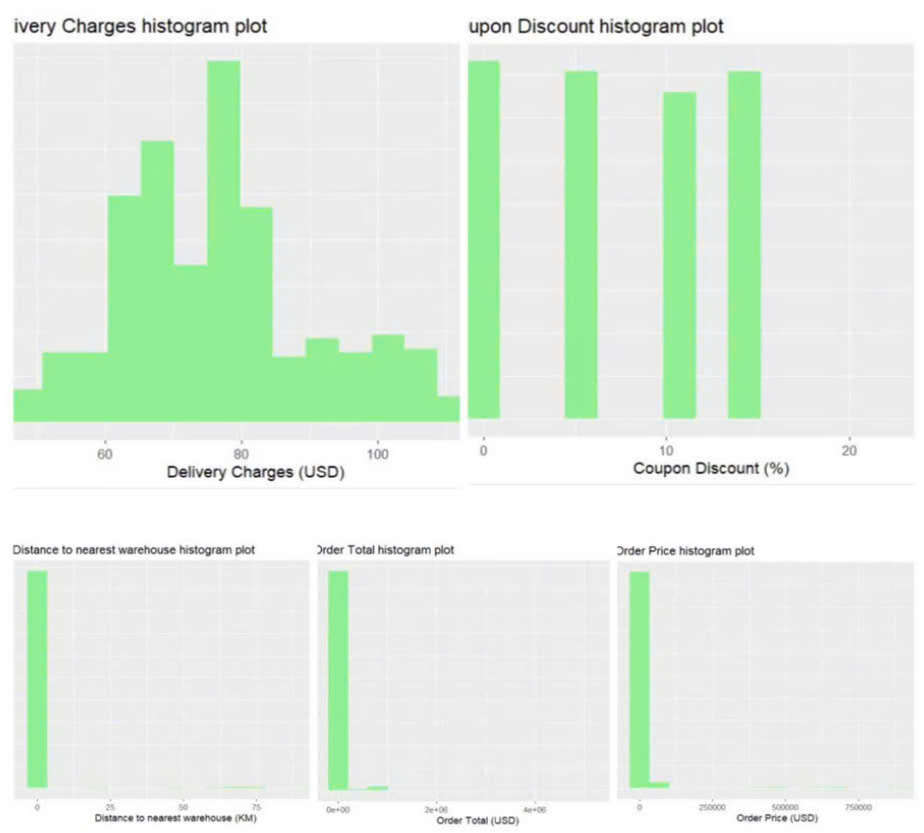
\includegraphics[width=0.7\linewidth]{graphics/bang7.jpg}
    \caption{Đồ thị Histogram của các biến liên tục}
  
\end{figure}
* Nhận xét: Ta nhận thấy rằng, từ kết quả đồ thị histogram cho thấy biến order\_total, order\_price, distance\_to\_nearest\_warehouse có phân phối lệch phải, với một cột cao ở phía bên trái. Điều này cho thấy hầu hết khách hàng chỉ chi tiêu ở mức thấp hơn, trong khi một số ít có tổng giá trị đơn hàng cao, tạo ra các điểm ngoại lệ. Phân phối lệch phải thường cho thấy  rằng có một số khách hang chi tiêu rất cao, điều này có thể ảnh hưởng đến quy mô hình hồi quy. Sau khi kiểm tra tỉ lệ khuyết nhỏ của các ngoại lai .Để xử lí tình trạng phân phối lệch phải này.\\
 -->Ta áp dụng xóa bỏ các ngoại lai  của order\_total, order\_price, distance\_to\_nearest\_warehouse.\\
 Dưới đây là hình ảnh sau khi xóa ngoại lai.
 \begin{figure}[H]
    \centering
    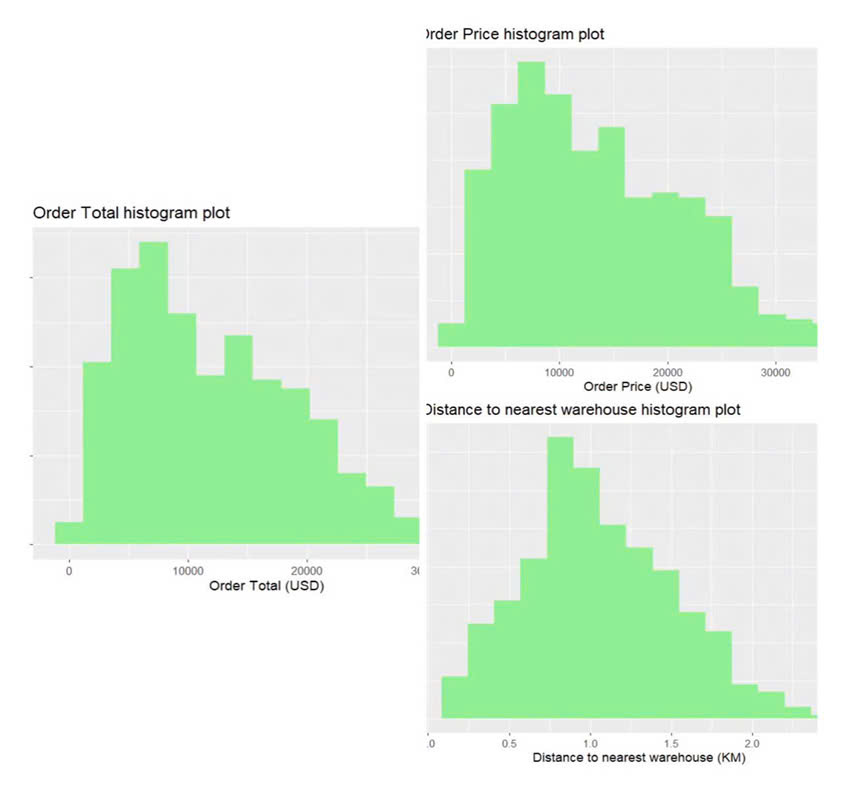
\includegraphics[width=0.7\linewidth]{graphics/bang8.jpg}
    \caption{Đồ thị Histogram của các biến liên tục đã xóa ngoại lai}
    
\end{figure}
\subsubsection{Đồ thị phân tần}
Ta so sánh  lần lượt từng order\_price, delivery\_charges, coupon\_discount, distance\_to\_nearest\_warehouse với order\_total.
\begin{figure}[H]
    \centering
    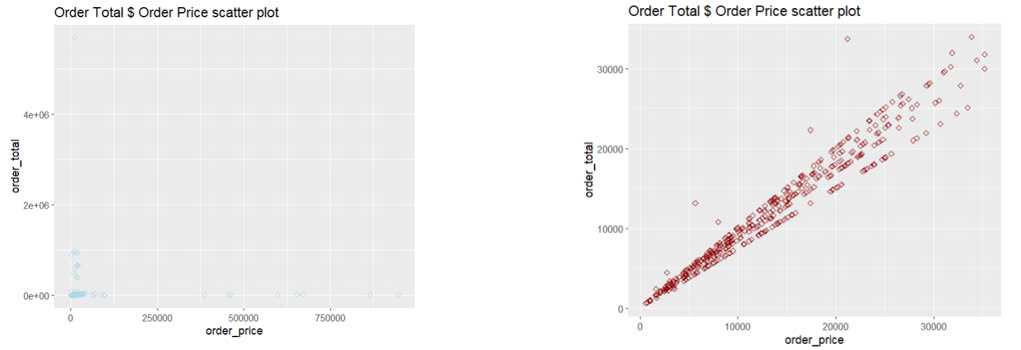
\includegraphics[width=0.8\linewidth]{graphics/bang9.jpg}
    \caption{Hình chưa xóa ngoại lai và đã xóa của order\_price}
 
\end{figure}
\begin{figure}[H]
    \centering
    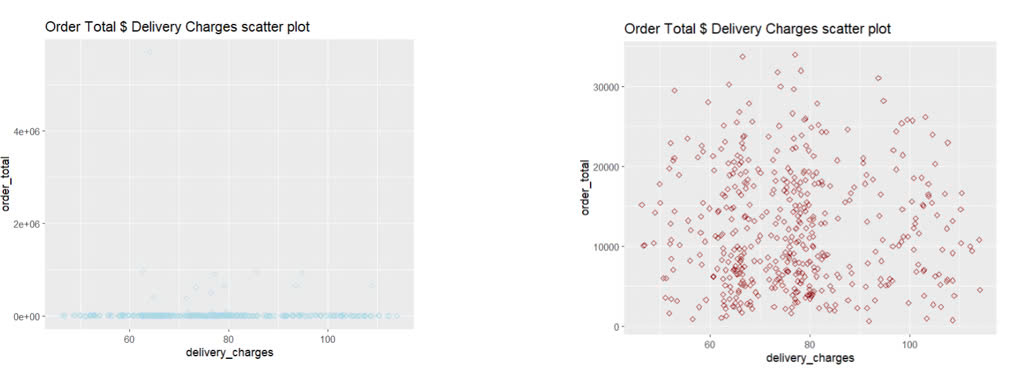
\includegraphics[width=0.8\linewidth]{graphics/bang10.jpg}
    \caption{Hình chưa xóa ngoại lai và đã xóa của delivery\_charges}
    
\end{figure}
\begin{figure}[H]
    \centering
    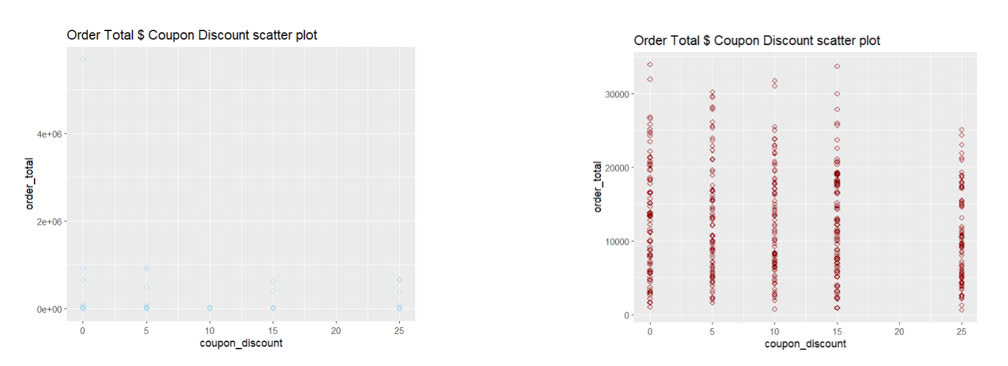
\includegraphics[width=0.8\linewidth]{graphics/bang11.jpg}
    \caption{Hình chưa xóa ngoại lai và đã xóa của coupon\_discount}
    
\end{figure}
\begin{figure}[H]
    \centering
    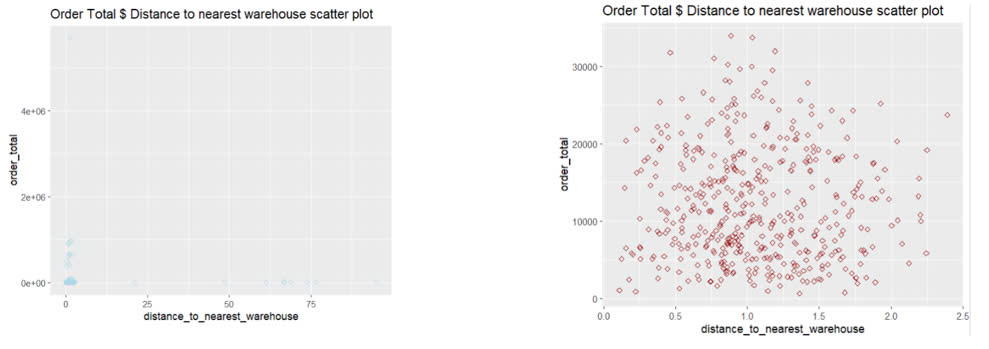
\includegraphics[width=0.8\linewidth]{graphics/bang12.jpg}
    \caption{Hình chưa xóa ngoại lai và đã xóa của distance\_to\_nearest\_warehouse}
 
\end{figure}
Với những hình ảnh có những chấm màu xanh là chưa xóa ngoại lai, còn những hình có chấm màu đỏ là đã xóa ngoại lai. \\
*Nhận xét: \\
•	Hai biến order\_price và coupon\_discount là 2 biến có ảnh hưởng tới order\_total hay còn gọi là có quan hệ tuyến tính.\\
•	Hai biến delivery\_charges và distance\_to\_nearest\_warehouse không có ảnh hưởng tới order\_total hay không có quan hệ tuyến tính.
\subsubsection{Phân tích biến định lượng bằng biểu đồ boxplot}
Ta phân tích biến order\_total theo các biến nearest\_warehouse, season, is\_expedited\_delivery, is\_happy\_customer.
\begin{figure}[H]
    \centering
    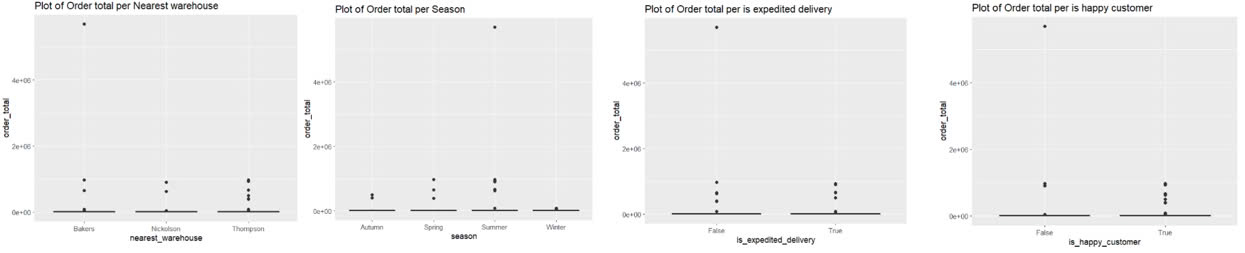
\includegraphics[width=1\linewidth]{graphics/bang13.jpg}
    \caption{Biểu đồ boxplot chưa xóa ngoại lai của các biến định lượng}
    
\end{figure}
\begin{figure}[H]
    \centering
    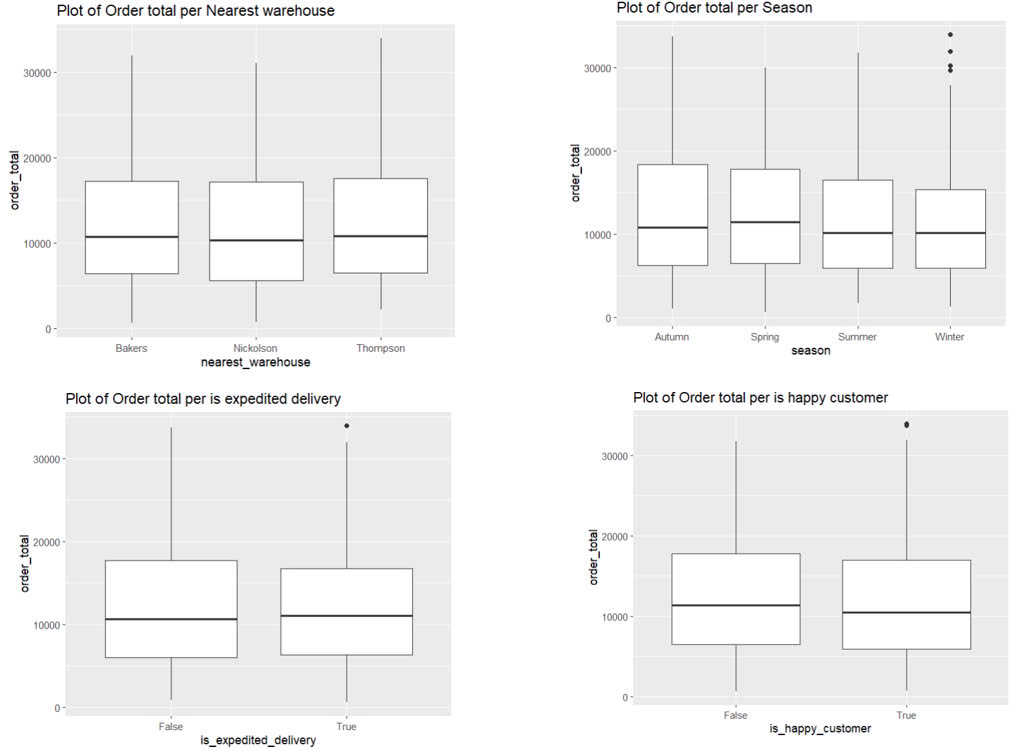
\includegraphics[width=1\linewidth]{graphics/bang14.jpg}
    \caption{Biểu đồ boxplot đã xóa ngoại lai của các biến định lượng}
    
\end{figure}
*Nhận xét: lần lượt cho  nearest\_warehouse, season, is\_expedited\_delivery, is\_happy\_customer.\\
•	Cả ba kho hàng (Bakers, Nickolson, Thompson) đều có phân bố tổng đơn hàng tương tự nhau, với các giá trị trung vị (median) gần như ngang bằng.\\
•	Phân bố giá trị order\_total khá đồng đều qua các mùa, tuy nhiên mùa Đông có một vài đơn hàng nổi bật với giá trị rất lớn.\\
•	Hình thức giao hàng nhanh dường như không có ảnh hưởng rõ rệt đến tổng giá trị đơn hàng trong phần lớn các trường hợp.\\
•	Trạng thái hài lòng của khách hàng không tạo ra sự khác biệt lớn trong tổng giá trị đơn hàng, nhưng nhóm khách hàng hài lòng có xu hướng chi tiêu nhiều hơn một chút và có thể thực hiện các đơn hàng có giá trị rất lớn (outliers).
\subsection{Bảng tương quan giữa các biến}
Bảng đánh giá tương quan trong đồ thị trên được sử dụng để hiểu rõ mối quan hệ giữa các biến số trong tập dữ liệu.
\begin{figure}[H]
    \centering
    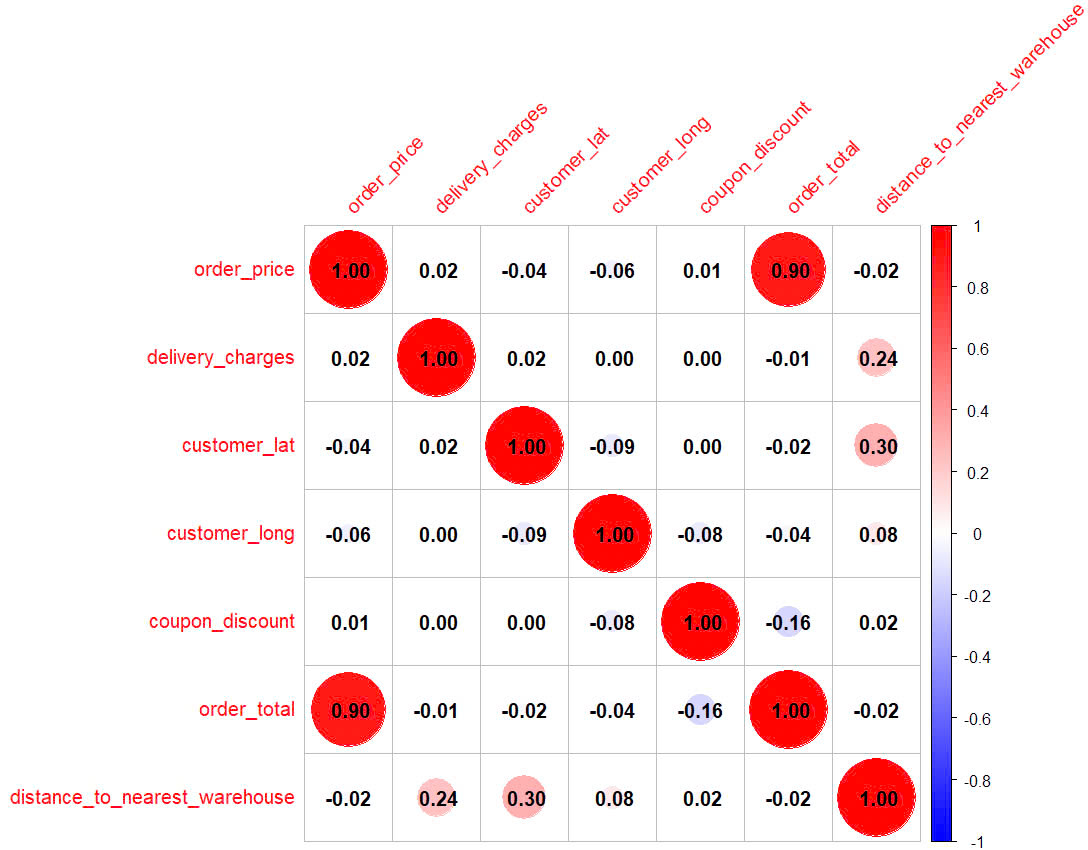
\includegraphics[width=0.8\linewidth]{graphics/tq.jpg}
    \caption{Biểu đồ tương quan của các biến}
    
\end{figure}

*Nhận Xét:

- order\_price và order\_total (tương quan: +0.90):
Đây là mối tương quan dương mạnh. Khi giá trị của order\_price tăng, order\_total cũng tăng mạnh theo và ngược lại. Điều này dễ hiểu vì order\_price là một thành phần chính của order\_total.

- distance\_to\_nearest\_warehouse và customer\_lat (+0.30):
Có mối tương quan dương trung bình giữa khoảng cách đến kho hàng và vĩ độ của khách hàng. Điều này có thể ngụ ý rằng vị trí kho hàng có xu hướng gần các khu vực cụ thể về mặt địa lý.

- distance\_to\_nearest\_warehouse và delivery\_charges (+0.24):
Mối tương quan dương nhẹ cho thấy khoảng cách đến kho hàng có tác động nhỏ đến chi phí giao hàng. Khoảng cách lớn hơn thường đi kèm với phí giao hàng cao hơn.

- order\_price và delivery\_charges (+0.02):
Hầu như không có mối liên hệ giữa giá trị đơn hàng và phí giao hàng. Điều này có thể chỉ ra rằng phí giao hàng không phụ thuộc vào giá trị đơn hàng mà dựa trên các yếu tố khác như khoảng cách hoặc chính sách giao hàng.

- coupon\_discount với hầu hết các biến khác (gần 0):
Mức giảm giá từ phiếu coupon không có mối liên hệ đáng kể với bất kỳ biến nào trong tập dữ liệu, kể cả order\_total. Điều này có thể ngụ ý rằng chiến lược giảm giá không ảnh hưởng rõ ràng đến hành vi mua sắm của khách hàng.
\section{Thống kê suy diễn}
\subsection{Phân tích phương sai một nhân tố (Single-factor ANOVA)}
\subsubsection{Dữ liệu}
	Y: 1 biến phụ thuộc,
	X: 1 biến nhân tố hay biến giải thích hay biến phân loại,
\subsubsection{mục tiêu}
	- Đánh giá biến X có ảnh hưởng đến biến phụ thuộc Y không?
\subsubsection{định nghĩa mô hình}
	$y_{ij}$=\mu + $\tau_{i} + $\varepsilon_ij$
	Trong đó:
	\mu: trung bình chung.
	$\tau_{i}$: tác động của nhóm thứ i.
	$\varepsilon_ij$: 

\subsection{Phân tích phương sai hai nhân tố (Two-factor ANOVA)}
\subsection{Hồi quy tuyến tính đa biến}
\section{Thảo luận}
Dưới góc độ phân tích thống kê, mô hình ANOVA (Phân tích phương sai) và mô hình hồi quy tuyến tính đa bội đều được sử dụng để khám phá mối quan hệ giữa các biến độc lập và biến phụ thuộc. Tuy nhiên, chúng có những điểm khác biệt cơ bản về mục đích và cách thức áp dụng. ANOVA thường được sử dụng khi các biến độc lập là các biến phân loại (như các nhóm hoặc điều kiện khác nhau) nhằm so sánh sự khác biệt trung bình của biến phụ thuộc giữa các nhóm này. Trong khi đó, hồi quy tuyến tính đa bội cho phép sử dụng cả các biến độc lập liên tục và phân loại, đồng thời cung cấp khả năng ước lượng tác động định lượng của từng biến độc lập lên biến phụ thuộc. Hồi quy tuyến tính đa bội còn cho phép kiểm soát nhiều yếu tố cùng lúc và khám phá các mối tương tác giữa các biến, điều mà ANOVA không thể làm được một cách trực tiếp. Bên cạnh đó, cả hai mô hình đều dựa trên các giả định về tính độc lập, phân phối chuẩn và phương sai đồng nhất, nhưng hồi quy tuyến tính đa bội thường linh hoạt hơn trong việc xử lý các tình huống phức tạp hơn trong nghiên cứu. Do đó, việc lựa chọn giữa ANOVA và hồi quy tuyến tính đa bội phụ thuộc vào bản chất của dữ liệu và mục tiêu phân tích cụ thể của nghiên cứu.
\pagebreak
\section{Nguồn dữ liệu và nguồn code}
Nguồn dữ liệu (dirty\_data.csv): \href{https://www.kaggle.com/datasets/muhammadshahrayar/transactional-retail-dataset-of-electronics-store?select=dirty_data.csv}{DATA}

Nguồn code R (link GG Drive): \href{https://drive.google.com/file/d/1jPlhtnxNBngjCb4IFFCHKuo0sPSkHAlP/view?usp=drive_link}{CODE}
\newpage
\addtocounter{page}{-1}
\cfoot{}  % Disable center footer (page number will be removed)
\lfoot{}  % Disable left footer
\rfoot{}  % Disable right footer
\renewcommand{\footrulewidth}{0pt}
\addcontentsline{toc}{section}{Tài liệu tham khảo}
\renewcommand{\refname}{Tài liệu tham khảo}
\begin{thebibliography}{9}
    \bibitem{r1}
    V.T. Nguyễn, \textit{Phân tích dữ liệu với R}, Nhà xuất bản Tổng hợp Thành phố HCM, 2014.
    \bibitem{r2}
    T. Tran, \textit{Lập trình R: tự học lập trình R từ cơ bản đến nâng cao}, Nhà xuất bản Đại học sư phạm HCM, 2019.
    \bibitem{r3}
    Nguyễn Đình Huy, \textit{BÀI TẬP XÁC SUẤT THỐNG KÊ}, NHÀ XUẤT BẢN ĐẠI HỌC QUỐC GIA TP. HỒ CHÍ MINH, 2023.
    \bibitem{r4}
    Nguyễn Đình Huy, \textit{GIÁO TRÌNH XÁC SUẤT VÀ THỐNG KÊ}, NHÀ XUẤT BẢN ĐẠI HỌC QUỐC GIA TP. HỒ CHÍ MINH, 2023.
\end{thebibliography}

\end{document}